\section{Controllability Analysis}

A full controllability analysis was performed on the system to establish whether:

\begin{enumerate}
	\item The system has acceptable set point tracking characteristics.
	\item The system has acceptable disturbance rejection characteristics.
\end{enumerate}

The method used is described in \textcite{skogestad}. 

\subsection{Minimal Realisation of the System}

The system written in the transfer function notation is in no danger of not being a minimal realizable system. It is only when the system is converted to state space notation it runs the risk of not being a minimal realization. 

When converting the transfer function model to a state space realisation of the system, it has to be noted that all dead time that is inherent to the system is ignored, as state space realizations cannot deal with dead time. The system was however converted to its state space realization, in order to cross check the calculated poles and zeros of the system.

The minimum state space realization of the system is given below.

\subsection{Functional Controllability}

The system has to be checked for functional controllability. This implies that outputs should be able to be controlled independently. There are two factors that have to be considered when checking for functional controllability of a system, namely

\begin{enumerate}
	\item There have to be at least as many inputs as there are outputs
	\item The rank of $G(s)$ should be greater than the number of outputs.
\end{enumerate} 

For consideration 1, mentioned above, the number of inputs and outputs in the system is equal. This criteria is therefore satisfied by the system.

For consideration 2, the minimum singular value (or $\underline{\sigma}$) of $G(j\omega)$ should be non-zero. In order to determine whether the system satisfies this criteria, all the singular values, of all the outputs were computed of a wide frequency range. A bode diagram displaying the result can be seem in Figure~\ref{fig:gs-singular-values}.

\begin{figure}
	\centering
	\includegraphics[width=0.7\linewidth]{"Figures/G(s) Singular Values"}
	\caption{The singular values of $G(j\omega)$.}
	\label{fig:gs-singular-values}
\end{figure}

As is clear from Figure~\ref{fig:gs-singular-values}, $\underline{\omega}$ never reaches zero, although it does approach zero as the frequency goes to infinity. 

Based on the above information, it can be concluded that the system is indeed functionally controllable. This implies that the system's rank is equal to the amount of outputs that the system has.

The current selected inputs and outputs can therefore be controlled with adequate independence. This further implies that outputs can return a response by some combination of the input variables.

A system that is functionally uncontrollable will have output responses remaining zero, whenever any combination of an input step function is applied to the system. This therefore results in an output that can in no way be controlled by the inputs, as the inputs do not effect the outputs at all.

\subsection{System Poles}
\label{sec:System Poles}
\subsubsection{Calculating the System Poles}

The poles of the system was calculated. The system has a total  number of 25 poles. Some of the poles calculated are listed in Table~\ref{tab: Poles of system}. These only contain the more interesting poles. Please refer to Figure~\ref{fig:polesandzeros} for the locations of all the calculated poles.

\begin{table}[H]
	\centering
	\caption{The poles of the system.}
	\begin{tabular}{ccc}
		\hline
		\textbf{Pole} & \textbf{Real Part} & \textbf{Imaginary Part} \\\hline
		$p_1$            & -0.31            & 0                       \\
		$p_2$            & -0.26            & 0                       \\
		$p_3$            & -0.20            & 0                 \\
		$p_4$            & -0.23            & 0                 \\
		$p_5$            & 0.036             & 0.23                  \\
		$p_6$            & 0.036             & -0.23   \\\hline             
	\end{tabular}
	\label{tab: Poles of system}
\end{table}

\subsubsection{Calculating the System Pole Directions}
\label{sec:Pole Directions}

The pole directions of the system was calculated by substituting the relevant pole values into $G(s)$ and calculating the input and output directions poles. This was only done for the poles occurring in the Right Hand Plane (RHP). The calculated pole directions are listed in Table~\ref{tab: Pole Directions of system}.

\begin{table}[H]
	\centering
	\caption{The pole directions of the system.}
	\begin{tabular}{ccc}
		\hline
		\textbf{Pole} & \textbf{Input Direction ($V$)} & \textbf{Output Direction ($U$)} \\\hline
		$p_5$            & $ \begin{bmatrix} -0.71 \\ 0.68 + 0.12j \\ 0.13 + 0.05j\end{bmatrix} $ & $ \begin{bmatrix} -0.19+0.22j \\ -0.79+0.53j \\ 0.02 -0.03j\end{bmatrix} $ \\
		$p_6$            & $ \begin{bmatrix} -0.71 \\ 0.68 - 0.12j \\ 0.13 -0.05j\end{bmatrix} $ & $ \begin{bmatrix} -0.19-0.22j \\ -0.79+0.53j \\ 0.02 - 0.03j\end{bmatrix} $ \\\hline             
	\end{tabular}
	\label{tab: Pole Directions of system}
\end{table}

\begin{table}[H]
	\centering
	\caption{The pole directions of the system in phasor notation.}
	\begin{tabular}{ccc}
		\hline
		\textbf{Pole} & \textbf{Input Direction ($V$)} & \textbf{Output Direction ($U$)} \\\hline
		$p_5$            & $ \begin{bmatrix} 0.71 \\ 0.69\angle10.1^{\circ} \\ 0.13\angle19.6^{\circ}\end{bmatrix} $ & $ \begin{bmatrix} 0.29\angle130.9^{\circ} \\ 0.96\angle146.0^{\circ} \\ 0.04\angle-48.9^{\circ}\end{bmatrix} $ \\
		$p_6$            & $ \begin{bmatrix} 0.71 \\ 0.69\angle-10.1^{\circ} \\ 0.13\angle-19.6^{\circ}\end{bmatrix} $ & $ \begin{bmatrix} 0.29\angle-130.9^{\circ} \\ 0.96\angle-146.0^{\circ} \\ 0.04\angle48.9^{\circ}\end{bmatrix} $ \\\hline             
	\end{tabular}
	\label{tab: Pole Directions of system Phasor Notation}
\end{table}


\subsubsection{Discussion of System Poles}

Most of the calculated system poles are in the open left hand plane (LHP). There is however one pair of complex poles that lie in the open RHP. These poles will cause instability when they are approached. To gain better understanding into the what causes the system to behave in this way, the pole directions were calculated in Section~\ref{sec:Pole Directions}. 

Using Table~\ref{tab: Pole Directions of system Phasor Notation} as reference the directions of the system in this unstable condition can be analysed. From the table it is clear that the unstable response exists whenever the variable $y_2$ (side stream composition) is increased by almost one unit. This cannot be done without effecting the output $y_1$, as it is increase by almost a third of a unit during this response. Only the temperature can remain relatively unaffected during the response. We also note that $y_1$ and $y_2$ are in phase with one another, while$y_3$ is out of phase the first two outputs.

Looking at the input directions in Table~\ref{tab: Pole Directions of system Phasor Notation}, it is clear that the described output is obtained from manipulation of $u_1$ and $u_2$. While $u_3$ is manipulated slightly, its amplitude is well below the amplitude of the other system inputs. We can therefore generalize and say that the pole exists when reflux flow rate is increased and side stream draw off flow rate is decreased by the same amount. One small thing to note, is that the input $u_1$ does not have a phasor notation, as it is not a complex variable.

From the above it is clear, that the side stream composition cannot stepped one unit by manipulating the side stream flow rate and reflux flow rate exclusively. This composition will have to be controlled other combinations of measured variable, for the system to remain stable.

From a production point of view, this will not likely pose to be problem, as it is not a scenario that is very likely to exist. As mentioned earlier, the main ethanol product is in the distillate of the column. The shift described by this pole, will decrease both the distillate and side stream flow rates, resulting in a plummeting production profit as the product streams are redirected to waste or downstream processing (the bottoms flow).
 

\subsection{System Zeros}
\label{sec:System Zeros}
\subsubsection{Calculating the System Zeros}

The system zeros were calculated. The system contains a total number of nine zeros, all of them located in the left hand plane (LHP). The system zeros are given in Table~\ref{tab: Zeros of system}.

\begin{table}[H]
	\centering
	\caption{The zeros of the system.}
	\begin{tabular}{ccc}
		\hline
		\textbf{Zero} & \textbf{Real Part} & \textbf{Imaginary Part} \\\hline
		$z_1$            & -0.3077            & 0                       \\
		$z_2$            & -0.2571            & 0                       \\
		$z_3$            & -0.2            & 0                  \\
		$z_4$            & -0.1493            & 0                 \\
		$z_5$            & -0.1227             & 0                  \\
		$z_6$            & -0.1157             & 0   \\
		$z_7$            & -0.1104             & 0   \\
		$z_8$            & -0.0917             & 0   \\
		$z_9$            & -0.0532             & 0   \\\hline             
	\end{tabular}
	\label{tab: Zeros of system}
\end{table}

Since all zeros are in the LHP, and will in no way cause limitations on the bandwidth or stability of the system, the directions of the zeros were not calculated.

\subsubsection{Discussion of System Zeros}

The system zeros exists for values of $s$ where the system $G(s)$ loses rank. The zeros calculated, are transmission zeros of the system as they do not relate to the zeros of the elements that make up the transfer function matrix $G(s)$. It is clear that there are no RHP zeros, and no further analysis of the zeros are required, as there are no limitations imposed by Left Hand Plane (LHP) zeros. 

LHP zeros will mostly cause high overshoots during control, but this does not pose as a stability concern for the system and will in no way limit the bandwidth of the system.

\begin{figure}[H]
	\centering
	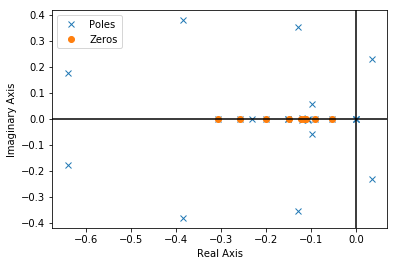
\includegraphics[width=0.7\linewidth]{Figures/Poles_and_Zeros}
	\caption{A graphical representation of the system's poles and zeros.}
	\label{fig:polesandzeros}
\end{figure}

\subsection{RGA Values of the System}
\label{sec:RGA Calculation}

The Routh Gain Array (RGA) of $G(j\omega)$ was calculated, for all values of $\omega$, where the frequency domain analysis held stable. This enables the analysis of RGA values not only for at the crossover frequencies, but at all other frequencies to thoroughly check for large RGA elements that will render a plant that is difficult to control. Due to dead time in the system, the frequency response of the RGA calculation tends to become severely unstable at higher frequencies. Luckily, spikes in the response will always tend to go downward, and the maximum RGA values can still be calculated. The calculated RGA analysis can be seen in Figure~\ref{fig:rga-values}.

\begin{figure}[H]
	\centering
	\includegraphics[width=0.7\linewidth]{"Figures/RGA Values"}
	\caption{The diagonal values of RGA matrix, $\Lambda$, over a wide range of frequencies.}
	\label{fig:rga-values}
\end{figure}

To verify that the off-diagonal values remain within acceptable ranges, the RGA of $G(0)$ and $G(j\omega)$ with $\omega = 10^{-1}$ was calculated. The two matrices calculated are

\begin{equation}
	\Lambda G(0) = \begin{bmatrix}
	2.11 & -0.84 & -0.26\\
	-0.59 & 1.67 & -0.08\\
	-0.52 & 0.17 & 1.34
	\end{bmatrix}
\end{equation}

\begin{equation}
\Lambda G(j10^{-1}) = \begin{bmatrix}
1.36 & -0.33 & -0.03\\
-0.37 & 1.34 & -0.03\\
0.02 & -0.02 & 1.00
\end{bmatrix}
\end{equation}

\subsection{Singular Values of the System}

\subsubsection{The Minimum Singular Value and Set-point Tracking}

The minimum singular value is a useful tool when doing controllability an analysis. The minimum singular value for this system is depicted in Figure~\ref{fig:gs-singular-values}.

The minimum singular value should be as large as possible, especially at frequencies where control is needed \parencite{skogestad}.

From Figure`\ref{fig:gs-singular-values}, it is clear that

\begin{equation}
	\label{eq: Min singular alue criteria}
	\underline{\sigma}(G(j\omega)) < 1 , \forall \omega
\end{equation}

This implies that it is not possible to make output changes of unit magnitude, by using inputs of unit magnitude for any input direction of $V$. 

This is bad from a controllability point of view, especially when considering set-point tracking. When tracking set-points, outputs ideally have to controlled by making single set-point changes. This enables the use of a decentralized controller. An example of such a controller (represented in a standard transfer function notation) is

\begin{equation}
	K(s) = \begin{bmatrix}
	\frac{K_1}{\tau_1s + 1} & 0 & 0\\
	 0 &\frac{K_2}{\tau_2s + 1} & 0\\
	 0 & 0 & \frac{K_3}{\tau_3s + 1}\\
	\end{bmatrix}
\end{equation} 

With the current plant configuration and design, the use of a decentralized controller is possible, but adequate set-point tracking will not be possible as the outputs will not reach the set-points on the high and/or low set-point values.

For example; when the temperature on tray \# 19 , $y_3$, is controlled between 88 and 96~$\celsius$, set-point tracking by manipulation of the stream feed pressure, $u_3$, will be acceptable (when considering a decentralized controller that contains an integral component). Acceptable set-point tracking includes: fast response time, elimination of error, robust responses. An adequately fast response time for this system will be around 45 minutes. With a high enough gain value, $K_{c3}$, this will be achieved. The integral component of the controller will eliminate the error completely over time, given that the integral component of the controller, $\tau_{c3}$, is large enough. Robust control will be achieved by tuning the controller values after initial implementation.

Now, when considering set-points on the outer limits of the control range for $y_3$, the control system will not perform acceptably. For instance when the set-point of $y_3$ is set to ranges 84 to 88 $\celsius$ or 96 to 100 $\celsius$, the response time of the set-point change may still be good, but the error will not be able to be cancelled. This is due to the minimum singular value of the system being smaller than 1. The unit change in the input, $u_3$, will not cause a unit change in the output, $y_3$. Since the system is scaled, this simply means that the outer set-points cannot be reached by only manipulating one input variable. 

The situation discussed above, only applies to the $y_3$ and $u_3$ control pairing. From Figure~\ref{fig:gs-singular-values}, it is clear that the criteria stated in Equation~\ref{eq: Min singular alue criteria} is satisfied for the $y_2$ and $u_2$ paring for all frequencies where $\omega<0.28$. Similarly, the criteria in Equation~\ref{eq: Min singular alue criteria} is satisfied in the $y_1$ and $u_1$ pairing for all frequencies where $\omega < 2.97$.

The are a few options for improvement and successful implementation of the control system. They are

\begin{enumerate}
	\item To implement a controller that is not decentralised. This controller can still control $y_1$ an $y_2$ using $u_1$ and $u_2$. $y_3$ will then be controlled by a combination of $u_3$ and $u_2$ (this follows from the RGA matrix analysis, where $u_1$ is negative with regard to $y_3$). The controller equation will then take the form of
	\begin{equation}
		K(s) = \begin{bmatrix}
		\frac{K_1}{\tau_1s + 1} & 0 & 0\\
		0 &\frac{K_2}{\tau_2s + 1} & 0\\
		0 & \frac{K_{3_1}}{\tau_{3_1}s + 1} & \frac{K_{3_2}}{\tau_{3_2}s + 1}\\
		\end{bmatrix}
	\end{equation}
	
	While this will ensure that acceptable set-point tracking of the bottom tray temperature is accomplished, there will be a loss in the performance and robustness of the control in the side-stream composition.
	
	\item Increase the size of the control valves controlling the stream pressure. This will increase the overall gain in the system, shifting the singular values in an upward direction. This will render acceptable set-point tracking of all parameters.
	
	\item Lower the required range wherein set-point tracking has to be performed. 
\end{enumerate}

More insight into the problem is gained when the different singular value directions are analysed. 

\subsubsection{Singular Value Directions}

The directions of the singular values are used to gain better understanding into how the three outputs are responsible for the overall system gain. The directions are calculate at both low and higher frequencies to analyse the behaviour at a wide range of frequencies. The two frequencies selected are $\omega = 0$ for low frequncies (or steady state values), and $\omega = 1$, which is the frequency at which the delays in the system causes the singular value to oscillate. The SVD for the low gain value is calculated as

\begin{equation}
	G(0) = 
	\underbrace{
		\begin{bmatrix}
		-0.38 & 0.88 & 0.26\\
		-0.92 & -0.39 & -0.03\\
		0.07 & -0.25 & 0.96\\
		\end{bmatrix}
	}_{U}
	\underbrace{
		\begin{bmatrix}
		12.9 & 0 & 0\\
		0 & 2.21 & 0\\
		0 & 0 & 0.56\\
		\end{bmatrix}
	}_{\Sigma}
	\underbrace{
		\begin{bmatrix}
		-0.64 & 0.51 & 0.57 \\
		0.73 & 0.62 & 0.23 \\
		0.22 & -0.59 & 0.77\\
		\end{bmatrix}
	}_{V^H}
\end{equation}

while the SVD for the higher gain is 

\begin{equation}
U(G(1j)) = 
	\begin{bmatrix}
	0.17\angle152^{\circ} & 0.96\angle-74.3^{\circ} & 0.22\angle116^{\circ}\\
	0.98\angle-86.4^{\circ} & 0.15\angle-132^{\circ} & 0.02\angle58.3^{\circ}\\
	0.0\angle-30.1^{\circ} & 0.23\angle100^{\circ} & 0.97\angle111^{\circ}\\
	\end{bmatrix}
\end{equation}

\begin{equation}
	\Sigma(G(1j)) =
		\begin{bmatrix}
		2.83 & 0 & 0\\
		0 & 0.59 & 0\\
		0 & 0 & 0.10\\
		\end{bmatrix}
\end{equation}

\begin{equation}
	V^H(G(1j)) = 
		\begin{bmatrix}
		0.77\angle0.0^{\circ} & 0.58\angle-180^{\circ} & 0.25\angle0.0^{\circ}\\
		0.63\angle-17.2^{\circ} & 0.65\angle-18.3^{\circ} & 0.41\angle166^{\circ}\\
		0.07\angle-134^{\circ} & 0.47\angle-121^{\circ} & 0.87\angle-117^{\circ}\\
		\end{bmatrix}
\end{equation}

\subsection{System Bandwidth}

The bandwidth of the system is the maximum frequency where sensible control can still be implemented. Mathematically it is where the sensitivity function of the system first crosses $1/\sqrt{2}$, or

\begin{equation}
	|S(j\omega)| = \frac{1}{\sqrt{2}}
\end{equation}

Since no controller is implemented as yet, there is no way of calculating the sensitivity function. As discussed in Section~\ref{sec:System Poles} and Section~\ref{sec:System Zeros}, there are no Right Hand Plane (RHP) zeros in this system. There are two RHP poles present, that will impose limitation on the on the system. The limitation imposed on the system are

\begin{enumerate}
	\item Limitations on the input usage. This constrains the amount of gain that can be applied to the system with a controller. In general
	
	\begin{equation}
		||KS||_{\infty} \geq ||u^H_p G_s(p)^{-1}||_2
	\end{equation}
	This is not entirely relevant to this report, as it entails the implementation of a controller. While this upper bound may be useful to assist with the design of the controller, the main focus of this report will remain on the controllability of the system.
	
	\item Limitations on the bandwidth. In short, the system has to react fast enough to avoid running into stability problems. The RHP pole therefore gives a minimum bound on the bandwidth (unlike RHP-zeros, which impose maximum bound constraints). According to \textcite{skogestad} the minimum closed loop bandwidth is 
	
	\begin{equation}
		\omega_B \geq 2|p|
	\end{equation}
	
	Using the equation the minimum bandwidth can be calculate to be $\omega_B = 0.46$. This gives a response time of less than 2.15 minutes.
\end{enumerate}

The system also contains a lot of dead time. There is dead time in each transfer function, as this is it is inherent to the fitting function used to build the model. There are constraints on the bandwidth due to this dead time. To visualize the dead time inherent to the system, please refer to Equation~\ref{eq:Deadtime Matrix}. This equation, simply named the dead time matrix, is a representation of the dead time elements ($\theta_{ij}$) for the respective transfer functions.

\begin{equation}
	\label{eq:Deadtime Matrix}
	\Theta = \begin{bmatrix}
	 2.6 & 6.5 & 9.2 \\
	 3.5 & 3.0 & 9.4 \\
	 1.0 & 1.2 & 1.0\\
	\end{bmatrix}
\end{equation} 

The lower bound time delay for each output (or contained within each row of $\Theta$) is of interest. This is because the minimum time for any input to effect the relevant output ($\theta_i^{min}$), can be seen as the delay that is pinned to output $y_i$. Alternatively this statement can be represented mathematically as 

\begin{equation}
	\theta_i^{min} = \min_j \theta_{ij}
\end{equation}

The bandwidth of input $u_i$ is then limited by the lower bound $1/\theta_i$. Table~\ref{tab:Bandwidths}, contains a summary of the bandwidth limitations of the system.

\begin{table}[H]
	\centering
	\begin{tabular}{ccc}
		\hline
		\textbf{Input} & \textbf{Theta} & \textbf{Bandwidth} \\
		\hline
		$y_1$             & 2.6            & 0.38               \\
		$y_2$             & 3.0              & 0.33               \\
		$y_3$             & 1.0              & 1.0                 \\\hline
	\end{tabular}
	\caption{Bandwidth limitations imposed by time delays.}
	\label{tab:Bandwidths}
\end{table}

While these limitations are in no way ideal, they do not pose to be a major threat for the control of the system. There are a few conclusions that can be drawn from this, namely

\begin{enumerate}
	\item When looking at Equation~\ref{eq:Deadtime Matrix} together with Section~\ref{sec:RGA Calculation}, it is clear that the diagonal elements that are paired in the RGA matrix, also contain the least amount of dead time. This is good, as it is obvious that you want to control a variable with an input that does not take long to effect the variable. Pairing of the variables are therefore made relatively straight forward.
	\item The delays imposed are not that significant when considering the desired response times for the control system. Required response times for the variables of the distillation column range between 30 and 60 minutes. The maximum delay calculated here (3 minutes), is relatively small and a low gain controller should be able to control the system with adequate performance. The performance of the system is discussed in more detail later in the report.
	\item Controlled variables $y_1$ and $y_2$ are more constrained by the RHP pole that exist than the delay that is inherent to these variables. Only $y_3$ is limited by the delay of the response. This is expected as the pole clearly influences $y_1$ and $y_2$ the most (Table~\ref{tab: Pole Directions of system}). $y_3$ also has the least amount of dead time, shortening the period wherein reasonable control can be expected.
\end{enumerate}

\subsection{Disturbance Rejection}

In order for the system to successfully reject disturbances, tight control and large bandwidths are required to when disturbances are large or "fast". 

To evaluate a MIMO system's ability to reject disturbances, the disturbance directions have to be evaluated (which is not the case when considering a SISO system). 

The model contains two disturbances, each having it's own associated direction. The disturbance directions are defined as

\begin{equation}
	y_d = \frac{1}{||g_d||_2}g_d
\end{equation}

where $g_d$ represents the effect of a single disturbance on the outputs ($y = g_dd$).

The disturbance directions for both disturbances were evaluated for all frequencies. The results can be seem in Figure~\ref{fig:disturbance-direction}.

\begin{figure}[H]
	\centering
	\includegraphics[width=0.7\linewidth]{"Figures/Disturbance Direction"}
	\caption{The disturbance directions as a function of frequency.}
	\label{fig:disturbance-direction}
\end{figure}

Now, following that the system has been scaled (Section~\ref{sec:Scaling}), we can say that the worst-case disturbance to be selected is $|d_i(\omega)| = 1$. Using this, and the fact that with feedback control we have $e = Sg_dd$, the disturbance performance objectives are then satisfied when

\begin{equation}
	||Sg_d||_{\infty} < 1
\end{equation}

Note that $S(s)$ could not actually be calculated. This is because no controller has yet been designed for the system. To gain better understanding of the disturbances in the system, a proportional decentralized controller with a gain of 1 (for all elemnts) was used.

\textcite{skogestad} used the above and derived tight bounds on the sensitivity function and loop gain for MIMO syste, considering the disturbance directions as well. For the system to adequately reject disturbances, we at least require that 

\begin{equation}
	\label{eq: Disturbance Criteria 1}
	\underline{\sigma}(S) < \frac{1}{||g_d||_2}
\end{equation}

Where $S$ is the sensitivity function of the transfer function model, or can be given mathematically as 

\begin{equation}
	S = (I + G)^{-1}
\end{equation}

for a negative feedback loop.

Equation~\ref{eq: Disturbance Criteria 1} can be represented graphically. The left-hand side and right-hand side of the equation was plotted for all values of $\omega$. The results are displayed in Figure~\ref{fig:disturbance-analysis-1}.

\begin{figure}[H]
	\centering
	\includegraphics[width=0.7\linewidth]{"Figures/Disturbance Analysis 1"}
	\caption{The disturbance directions with respect to the singular values of the sensitivity of $G(s)$, $S(s)$.}
	\label{fig:disturbance-analysis-1}
\end{figure}

From Figure~\ref{fig:disturbance-analysis-1}, it is clear that, based on the criteria stated in Equation~\ref{eq: Disturbance Criteria 1}, there may be some problems regarding disturbance rejection (especially at low frequencies). To share more light on the causes of the problem, an more in depth analysis is conducted below.

\subsection{Disturbances and Input Saturation}

\subsubsection{Analysis for Perfect Control}
Here it is asked whether disturbance rejection is possible, without input saturation \newline($||u||<1$). There are two methods of evaluating this, by use of

\begin{enumerate}
	\item The max-norm.
	\item The two norm.
\end{enumerate}

As the system is square, the max-norm can be used to analyse this plant. Disturbances are analysed separately, and combined to gain full understanding of how the disturbances will effect the controller input. 

When considering single disturbances, input saturation is avoided (and perfect control is achieved) when

\begin{equation}
	||G^{-1} g_d||_{max} < 1 
\end{equation} 

and when considering simultaneous disturbances the requirement can be rewritten to

\begin{equation}
	||G^{-1} G_d||_{i\infty} < 1
\end{equation} 

where $||\cdot||_{i\infty}$ is the induced max-norm defined as

\begin{equation}
	||A||_{i\infty} = \max_{j} \Big(\sum_{i}|a_{ij}|\Big)
\end{equation}

The criteria stated above is displayed in Figure~\ref{fig:disturbance-analysis-2-max-norm}.

\begin{figure}[H]
	\centering
	\includegraphics[width=0.7\linewidth]{"Figures/Disturbance Analysis 2 Max Norm"}
	\caption{The effect of disturbances on input saturation.}
	\label{fig:disturbance-analysis-2-max-norm}
\end{figure}

From Figure~\ref{fig:disturbance-analysis-2-max-norm}, it is clear that perfect control is not possible for either disturbance, or even for a combination of both. The disturbance $d_2$ is the most problematic, as the disturbance causes $||G^{-1}g_d||_{\infty}||$ to be greater than 1 for all values of frequency. Perfect control of this disturbance is not possible. 

Input saturation is therefore unavoidable. This does not necessarily mean that the plant is uncontrollable with regard to disturbance rejection. An analysis for acceptable disturbance rejection with regard to input saturation has to be performed.

\subsubsection{Analysis for Acceptable Control}
\label{sec:Analysis for acceptable control:disturbances}
 Acceptable control exists when, for the response $e = Gu+G_dd$ it is possible achieve $||r||\leq1$ for any $||d||\leq1$ using inputs $||u||\leq1$. Only the max-norm is used in this section. The conditions resulting from the analysis are for achieving $||e||\leq1$ (the minimum requirement).
 
 The criteria derived by \textcite{skogestad} for system to exhibit acceptable control characteristics is given as
 
 \begin{equation}
 	\label{eq:Input saturation of disturbances}
 	\sigma_i(G) \geq |u_i^Hg_d| -1 \textrm{, at frequencies where } |u_i^Hg_d|>1
 \end{equation}
 
 Figure~\ref{fig:Input Saturation 1}, Figure~\ref{fig:Input Saturation 2} and Figure~\ref{fig:Input Saturation 3} are the graphical representations of the criteria stated in Equation~\ref{eq:Input saturation of disturbances} for the three different input directions. The effect of both disturbances are plotted against the singular value for the specific input. This will help to gain insight into the way that disturbances effect the input values to the controller.
 
 \begin{figure}[H]
 	\centering
 	\begin{minipage}{.48\textwidth}
 		\centering
 		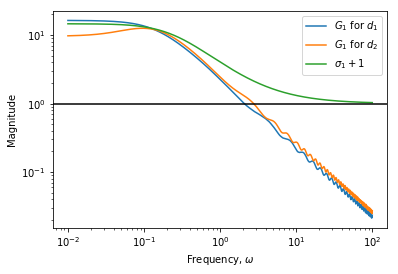
\includegraphics[width=\linewidth]{Figures/InputSaturation1}
 		\captionof{figure}{Graphical representation of criteria outlined in Equation~\ref{eq:Input saturation of disturbances}, for $e_1$}
 		\label{fig:Input Saturation 1}
 	\end{minipage}%
 	\hfill
 	\begin{minipage}{.48\textwidth}
 		\centering
 		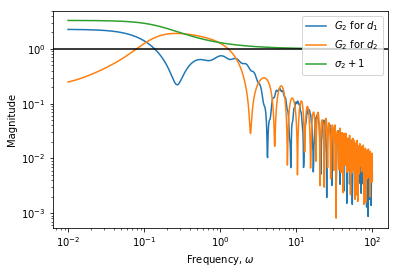
\includegraphics[width=\linewidth]{Figures/InputSaturation2}
 		\captionof{figure}{Graphical representation of criteria outlined in Equation~\ref{eq:Input saturation of disturbances}, for $e_2$}
 		\label{fig:Input Saturation 2}
 	\end{minipage}
 \end{figure}

 \begin{figure}[H]
	\centering
	\begin{minipage}{.48\textwidth}
		\centering
		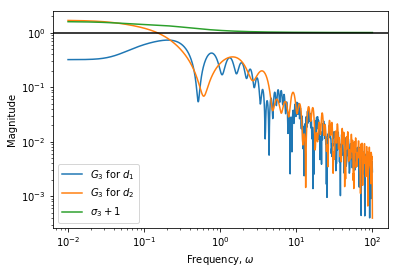
\includegraphics[width=\linewidth]{Figures/InputSaturation3}
		\captionof{figure}{Graphical representation of criteria outlined in Equation~\ref{eq:Input saturation of disturbances}, for $e_3$}
		\label{fig:Input Saturation 3}
	\end{minipage}%
	\hfill
	\begin{minipage}{.48\textwidth}
		\centering
		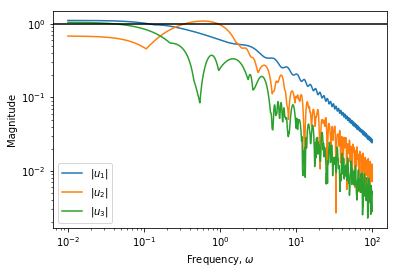
\includegraphics[width=\linewidth]{Figures/Input_Requirements}
		\captionof{figure}{The required controller input values for the worst case }
		\label{fig:Input Requirements}
	\end{minipage}
\end{figure}

When considering Figure~\ref{fig:Input Saturation 1}, it is clear that the input into the controller (controlling $y_1$) is saturated at low frequencies. This is due to the effects that $d_1$ has on the system. It is clear that a maximum change in the feed flow rate, will result in the reflux flow rate flow being saturated. This translates to a fully open or fully closed control valve in this section of the plant. There are two solutions to the problem, namely

\begin{enumerate}
	\item Install a bigger control valve (and therefore line size) on the reflux stream. This change will impact the mathematical model by changing the gain and response times in the first row of transfer function matrix $G(s)$. This speed up the dynamics of the system, and result in higher minimum singular values for $S(s)$, especially at low frequencies where the problem is experienced. Better disturbance rejection will result.
	
	\item Lower the maximum designed for disturbance size. This can be done by tighter control upstream from the distillation column (by the flow regulator/controller indicated in Figure~\ref{fig:PFD}).
	
\end{enumerate}   

Both actions will take considerable time to implement, as the effect of tighter flow control will effect the reactor vessel's control as well. A bigger, or more sophisticated control valve, will have a installation cost, as well as a downtime, as well as recommissioning of the system, production cost implication. 

From Figure~\ref{fig:Input Saturation 2} it is clear that acceptable control is possible, since the second input to the controller is saturated by neither disturbance changes (for all frequencies).

Regarding Figure~\ref{fig:Input Saturation 3}, it is clear that disturbance rejection is again not acceptable, as the third input to the controller ($e_3$) is saturated when disturbance $d_2$ is at it's maximum feed value. When relating back to the physical process, this means that the stream pressure control valve, fully closes when the feed temperature rises to 106 $^{\circ}$F or fully opens when the feed temperature drops to 58 $^{\circ}$F. To solve this problem there again exists a few solutions, namely

\begin{enumerate}
	\item Increase the size of the control valve. When doing this, it is imperative that the compressors in the stream line's design also be reviewed, as it may be required that a higher stream flow rate be required at the lowest disturbance value. The major downside of this option, is that there is no compensation for when the feed temperature rises to the maximum disturbance value. Even the bigger control valve will still fully close.
	\item Decrease the disturbance limit values. This is again the most straightforward method to increase the effectiveness of disturbance rejection over the distillation column. This can be done by implementing tighter control over the feed heat exchanger unit (indicated in Figure~\ref{fig:PFD}). Methods to implement tighter control will be to increase the controller gain of the unit (an decreasing the amount of integral control). Implementing a feed forward controller on the heat exchanger unit by adding the working fluid's temperature as measured variable is another option (although this will not be the most cost effective solution).
	\item Change the controlled variable $y_3$. By changing the controlled variable $y_3$ from the temperature on tray \#19, to the boil-up ratio will reduce the response time in dynamics of the third row in $G(s)$. This will lead to higher singular values in $S(s)$, especially at low frequencies, and disturbance rejection performance criteria will be met. This solution has the downside that the bottoms composition will not be controlled directly. Since the production is more interested in the quality of the distillate composition (as this is where the ethanol product is), this is not a major loss and the solution can be considered. A full controllability analysis will have to be conducted on the new system if this is the chosen solution, as the dynamics of the whole MIMO transfer function model will change.
\end{enumerate}

Figure~\ref{fig:Input Requirements} illustrates the required input variables ($u_i$) for maximum disturbance rejection. The figure reiterates the problems experienced in Figure~\ref{fig:Input Saturation 1} and Figure~\ref{fig:Input Saturation 3}, where the inputs required for disturbance rejection will saturate the controller.  

